%%%%%%%%%%%%%%%%%%%%%%%%%%%%%%%%%%%%%%%%%
% Programming/Coding Assignment
% LaTeX Template
%
% This template has been downloaded from:
% http://www.latextemplates.com
%
% Original author:
% Ted Pavlic (http://www.tedpavlic.com)
%
% Note:
% The \lipsum[#] commands throughout this template generate dummy text
% to fill the template out. These commands should all be removed when 
% writing assignment content.
%
% This template uses a Perl script as an example snippet of code, most other
% languages are also usable. Configure them in the "CODE INCLUSION 
% CONFIGURATION" section.
%
%%%%%%%%%%%%%%%%%%%%%%%%%%%%%%%%%%%%%%%%%

%----------------------------------------------------------------------------------------
%	PACKAGES AND OTHER DOCUMENT CONFIGURATIONS
%----------------------------------------------------------------------------------------

\documentclass{article}

\usepackage{fancyhdr} % Required for custom headers
\usepackage{lastpage} % Required to determine the last page for the footer
\usepackage{extramarks} % Required for headers and footers
\usepackage[usenames,dvipsnames]{xcolor} % Required for custom colors
\usepackage{graphicx} % Required to insert images
\usepackage{listings} % Required for insertion of code
\usepackage{courier} % Required for the courier font
\usepackage{tikz}
\usepackage{capt-of}
\usetikzlibrary{automata,positioning}
% Margins
\topmargin=-0.45in
\evensidemargin=0in
\oddsidemargin=0in
\textwidth=6.5in
\textheight=9.0in
\headsep=0.25in

\linespread{1.1} % Line spacing

% Set up the header and footer
\pagestyle{fancy}
\lhead{\hmwkAuthorName} % Top left header
\chead{\hmwkClass: \hmwkTitle} % Top center head
\rhead{\firstxmark} % Top right header
\lfoot{\lastxmark} % Bottom left footer
\cfoot{} % Bottom center footer
\rfoot{Page\ \thepage\ of\ \protect\pageref{LastPage}} % Bottom right footer
\renewcommand\headrulewidth{0.4pt} % Size of the header rule
\renewcommand\footrulewidth{0.4pt} % Size of the footer rule

\setlength\parindent{0pt} % Removes all indentation from paragraphs

%----------------------------------------------------------------------------------------
%	CODE INCLUSION CONFIGURATION
%----------------------------------------------------------------------------------------

\definecolor{MyDarkGreen}{rgb}{0.0,0.4,0.0} % This is the color used for comments
\lstloadlanguages{Python}
\lstset{language=Python,
        frame=single, % Single frame around code
        basicstyle=\small\ttfamily, % Use small true type font
        commentstyle=\usefont{T1}{pcr}{m}{sl}\color{MyDarkGreen}\small, % Comments small dark green courier font
        stringstyle=\color{Purple}, % Strings are purple
        showstringspaces=false, % Don't put marks in string spaces
        tabsize=5, % 5 spaces per tab
        morecomment=[l][\color{Blue}]{...}, % Line continuation (...) like blue comment
        numbers=left, % Line numbers on left
        firstnumber=0, % Line numbers start with line 0
        numberstyle=\tiny\color{Blue}, % Line numbers are blue and small
        stepnumber=1 % Line numbers go in steps of 1
}

% Creates a new command to include a perl script, the first parameter is the filename of the script (without .pl), the second parameter is the caption
\newcommand{\pythonscript}[2]{
\begin{itemize}
\item[]\lstinputlisting[caption=#2,label=#1]{#1.py}
\end{itemize}
}

\def\code#1{\texttt{#1}} % Added by GZZ
%----------------------------------------------------------------------------------------
%	DOCUMENT STRUCTURE COMMANDS
%	Skip this unless you know what you're doing
%----------------------------------------------------------------------------------------

% Header and footer for when a page split occurs within a problem environment
\newcommand{\enterProblemHeader}[1]{
\nobreak\extramarks{#1}{#1 continued on next page\ldots}\nobreak
\nobreak\extramarks{#1 (continued)}{#1 continued on next page\ldots}\nobreak
}

% Header and footer for when a page split occurs between problem environments
\newcommand{\exitProblemHeader}[1]{
\nobreak\extramarks{#1 (continued)}{#1 continued on next page\ldots}\nobreak
\nobreak\extramarks{#1}{}\nobreak
}

\setcounter{secnumdepth}{0} % Removes default section numbers
\newcounter{homeworkProblemCounter} % Creates a counter to keep track of the number of problems

\newcommand{\homeworkProblemName}{}
\newenvironment{homeworkProblem}[1][Problem \arabic{homeworkProblemCounter}]{ % Makes a new environment called homeworkProblem which takes 1 argument (custom name) but the default is "Problem #"
\stepcounter{homeworkProblemCounter} % Increase counter for number of problems
\renewcommand{\homeworkProblemName}{#1} % Assign \homeworkProblemName the name of the problem
\section{\homeworkProblemName} % Make a section in the document with the custom problem count
\enterProblemHeader{\homeworkProblemName} % Header and footer within the environment
}{
\exitProblemHeader{\homeworkProblemName} % Header and footer after the environment
}

\newcommand{\problemAnswer}[1]{ % Defines the problem answer command with the content as the only argument
\noindent\framebox[\columnwidth][c]{\begin{minipage}{0.98\columnwidth}#1\end{minipage}} % Makes the box around the problem answer and puts the content inside
}

\newcommand{\homeworkSectionName}{}
\newenvironment{homeworkSection}[1]{ % New environment for sections within homework problems, takes 1 argument - the name of the section
\renewcommand{\homeworkSectionName}{#1} % Assign \homeworkSectionName to the name of the section from the environment argument
\subsection{\homeworkSectionName} % Make a subsection with the custom name of the subsection
\enterProblemHeader{\homeworkProblemName\ [\homeworkSectionName]} % Header and footer within the environment
}{
\enterProblemHeader{\homeworkProblemName} % Header and footer after the environment
}

%----------------------------------------------------------------------------------------
%	NAME AND CLASS SECTION
%----------------------------------------------------------------------------------------

\newcommand{\hmwkTitle}{CiScal Compiler} % Assignment title
\newcommand{\hmwkDueDate}{Monday,\ March\ 13,\ 2017} % Due date
\newcommand{\hmwkClass}{MYY802} % Course/class
\newcommand{\hmwkClassTime}{} % Class/lecture time
\newcommand{\hmwkClassInstructor}{George Manis} % Teacher/lecturer
\newcommand{\hmwkAuthorName}{G.Zachos, A.Konstantinidis} % Your name

%----------------------------------------------------------------------------------------
%	TITLE PAGE
%----------------------------------------------------------------------------------------

\title{
\vspace{2in}
\textmd{\textbf{\hmwkClass:\ \hmwkTitle}}\\
\normalsize\vspace{0.1in}\small{Due\ on\ \hmwkDueDate}\\
\vspace{0.1in}\large{\textit{\hmwkClassInstructor}}
\vspace{3in}
}

\author{\textbf{\hmwkAuthorName}}
\date{March 5, 2017} % Insert date here if you want it to appear below your name

%----------------------------------------------------------------------------------------

\setcounter{secnumdepth}{3}

\begin{document}

\maketitle

%----------------------------------------------------------------------------------------
%	TABLE OF CONTENTS
%----------------------------------------------------------------------------------------

\newpage
\tableofcontents
\newpage

%----------------------------------------------------------------------------------------
%	Intro
%----------------------------------------------------------------------------------------

\section{About}

\subsection{CiScal language}
CiScal is a minimal programming language that has borrowed many of its characteristics from C and Pascal.
In contrast to its limited capabilities, the development process of a CiScal compiler is quite interesting.

In general, the language does support the following features:
\begin{itemize}
 \item Numeric (integer) constans between -32768 and 32767
 \item \code{if-else}, \code{do-while}, \code{while}, \code{select} and assignment statements
 \item Relational and arithmetic expressions
 \item Definition of functions and procedures; both nested and not
 \item Parameter passing by reference and by value
 \item Recursive function/procedure calls
\end{itemize}

For more information on CiScal capabilities please refer to \code{ciscal-grammar.pdf}

\vspace{0.5cm}
On the other hand, the features below are not supported:
\begin{itemize}
 \item \code{for}-loops
 \item Real numbers
 \item Characters and strings
\end{itemize}


\subsection{CiScal Compiler}
CiScal Compiler (CSC) was developed during the MYY802 - Compilers course at the Department of
Computer Science and Engineering, University of Ioannina. It is written in Python 3 and serves
to transform CiScal source code to MIPS Assembly code.

\subsubsection{Using the compiler}
To learn how to use CSC run \verb|./csc.py| and the information below will be printed to console:

\begin{verbatim}
  Usage: ./csc.py [OPTIONS] {-i|--input} INFILE
  Available options:
          -h, --help                Display this information
          -v, --version             Output version information
          -I, --interm              Keep intermediate code (IC) file
          -C, --c-equiv             Keep IC equivalent in C lang file
          --save-temps              Equivalent to -IC option
          -o, --output OUTFILE      Place output in file: OUTFILE
\end{verbatim}

\pagebreak


%----------------------------------------------------------------------------------------
%	Deliverables
%----------------------------------------------------------------------------------------

\section{Deliverables}

\begin{itemize}
 \item 1st Phase (10\%)
 \begin{itemize}
  \item Lexical Analysis
  \item Syntax Analysis
 \end{itemize}

 \item 2nd Phase (30\%)
 \begin{itemize}
  \item Intermediate Code Generation
 \end{itemize}
 
 \item 3rd Phase (10\%)
 \begin{itemize}
  \item Semantic Analysis
  \item Symbol Table
 \end{itemize}

 \item 4th Phase (50\%)
 \begin{itemize}
  \item Final Code Generation (30\%)
  \item Project Report (20\%)
 \end{itemize}
\end{itemize}


%----------------------------------------------------------------------------------------
%	Error Handling
%----------------------------------------------------------------------------------------

\section{Error Handling}

To simplify display of error messages, the following functions have been defined:
\begin{itemize}
 \item \code{perror\_exit()}: Prints an error message to stderr and program exits
 \item \code{perror()}: Prints an error message to stderr
 \item \code{pwarn()}: Prints a warning to stderr
 \item \code{perror\_line\_exit(ec, lineno, charno, ...)}: Prints line \underline{lineno}
       of the inputfile to stderr with character \underline{charno} highlighted and along
       with and error message. Finally the program exits.
\end{itemize}



\pagebreak

%----------------------------------------------------------------------------------------
%	Lexical Analyzer
%----------------------------------------------------------------------------------------

% To have just one problem per page, simply put a \clearpage after each problem

\section{Lexical Analyzer}

%\subsection{Finite Automata}
The Finite-State Machine (FSM) diagram in Figure \ref{fig:fsm} is a partial graphical representation of the
finite automata implemented in the \code{lex()} function and which is used to convert the input
sequence of characters into a sequence of language tokens. In addition to the states shown below,
there are fourteen (14) more accepting states that correspond to characters: '\code{+}', '\code{-}', '\code{*}', 
'\code{/}', '\code{=}', '\code{,}', '\code{;}', '\code{\{}', '\code{\}}', '\code{(}', '\code{)}', 
'\code{[}', '\code{]}' and '\code{eof}'. Transition to these states is triggered only from initial state $s_0$.
\vspace{1cm}

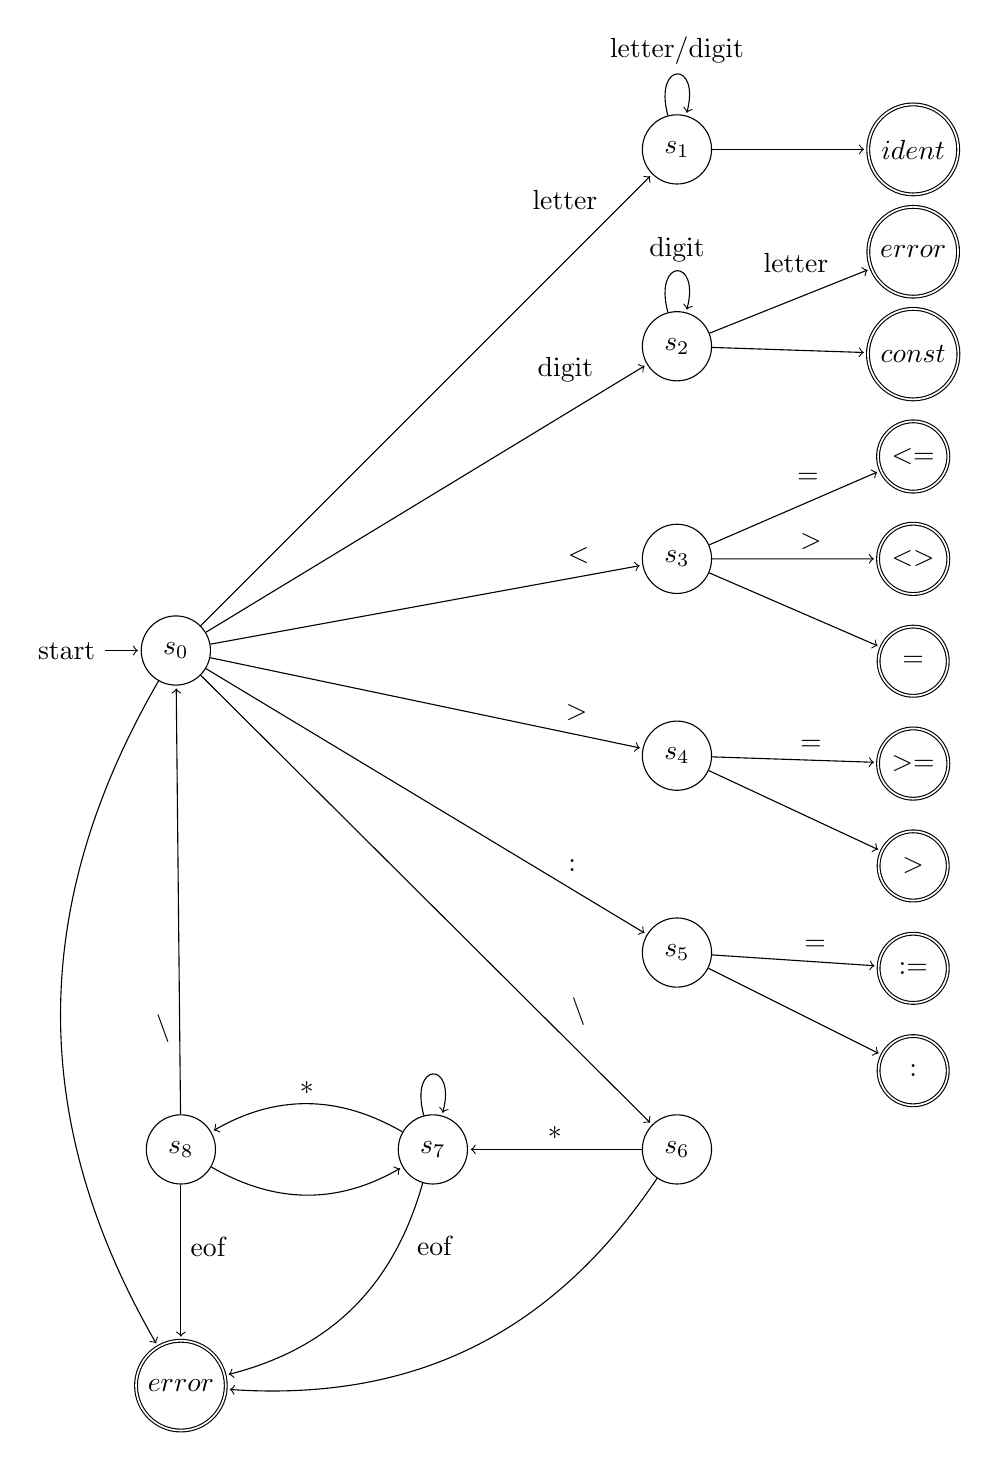
\begin{tikzpicture}[shorten >=1pt,node distance=3cm,on grid,auto]
  \tikzstyle{every state}=[align=center]
  \node[state,initial] (s_0)   {$s_0$};
  \node[state] (s_1) [above right=9cm of s_0] {$s_1$};
  \node[state, accepting] (ident) [right=of s_1] {$ident$};
  \node[state] (s_2) [below=2.5cm of s_1] {$s_2$};
  \node[state, accepting] (err_0) [below =1.3cm of ident] {$error$};
  \node[state, accepting] (const) [below =1.3cm of err_0] {$const$};
  \node[state] (s_3) [below=2.7cm of s_2] {$s_3$};
  \node[state, accepting] (leq) [below =1.3cm of const] {$<=$};
  \node[state, accepting] (neq) [below =1.3cm of leq] {$<>$};
  \node[state, accepting] (eq) [below =1.3cm of neq] {$=$};
  \node[state] (s_4) [below=2.5cm of s_3] {$s_4$};
  \node[state, accepting] (geq) [below =1.3cm of eq] {$>=$};
  \node[state, accepting] (gtr) [below =1.3cm of geq] {$>$};
  \node[state] (s_5) [below=2.5cm of s_4] {$s_5$};
  \node[state, accepting] (become) [below =1.3cm of gtr] {$:=$};
  \node[state, accepting] (colon) [below =1.3cm of become] {$:$};
  \node[state] (s_6) [below=2.5cm of s_5] {$s_6$};
  \node[state] (s_7) [left=3.1cm of s_6] {$s_7$};
  \node[state] (s_8) [left=3.2cm of s_7] {$s_8$};
  \node[state, accepting] (err_1) [below=3cm of s_8] {$error$};
    \path[->] 
    (s_0) edge node [pos = 0.9] {letter} (s_1)
          edge node [pos = 0.9] {digit} (s_2)
          edge node [pos = 0.9] {$<$} (s_3)
          edge node [pos = 0.8] {$>$} (s_4)
          edge node [pos = 0.8] {$:$} (s_5)
          edge node [pos = 0.8] {$\backslash$} (s_6)
          edge [bend right] node {} (err_1)
    (s_1) edge [loop above] node {letter/digit} (s_1)
          edge node {} (ident)
    (s_2) edge [loop above] node {digit} (s_2)
          edge node [pos= 0.5, below] {} (const)
          edge node [pos= 0.8] {letter} (err_0)
    (s_3) edge node [pos = 0.7] {$=$} (leq)
          edge node [pos = 0.6] {$>$} (neq)
          edge node {} (eq)
    (s_4) edge node [pos = 0.6] {$=$} (geq)
          edge node {} (gtr)
    (s_5) edge node [pos = 0.5] {$=$} (become)
          edge node {} (colon)
    (s_6) edge node [above] {$*$} (s_7)
          edge [bend left] node {} (err_1)
    (s_7) edge [loop above] node {} (s_7)
          edge [bend right] node [above] {$*$} (s_8)
          edge [bend left] node [pos = 0.15] {eof} (err_1)
    (s_8) edge node [pos = 0.2] {$\backslash$} (s_0)
          edge [bend right] node {} (s_7)
          edge node [pos = 0.4, right] {eof} (err_1);
\end{tikzpicture}
\captionof{figure}{Partial FSM diagram of lexical analyzer's finite automata}\label{fig:fsm}

\pagebreak

\subsection{Implementation details}

\subsubsection{Custom Classes}
During the Implementation of the lexical analyzer, a couple of classes were defined.
The first class defined was the \code{TokenType} class which is an enumeration that maps token
types to enumerated constants. The other class was the \code{Token} class and was defined to group
all useful information related to a token and that should be available to the syntax analyzer. 
This information includes:
\begin{itemize}
 \item \code{tktype}: token type (attribute of the \code{TokeType} enumeration)
 \item \code{tkval}: the actual token value
 \item \code{tkl}: the line of the input file that the token was found
 \item \code{tkc}: the offset of the token's first character from the start of line \code{tkl}
\end{itemize}

% \pythonscript{token-class}{Token Class}

\subsubsection{Data Structures}
The \code{token} dictionary maps actual keyword values to the corresponding \code{TokenType} 
attributes and serves code simplicity.
\pythonscript{token-dict}{Token type/value dictionary}

\subsubsection{Return value}
The \code{lex()} function returns an object of type \code{Token} to the syntax analyzer.

%----------------------------------------------------------------------------------------
%	Syntax Analyzer
%----------------------------------------------------------------------------------------

\section{Syntax Analyzer}

In order for the syntax analysis to take place, a function for each grammar rule was defined. 
In the \code{syntax\_analyzer()} function, the global variable \code{token} is assigned the
\code{Token} class instance returned by the first call to \code{lex()}. Then the \code{program()}
function that implements the \code{<PROGRAM>} grammar rule is called and upon success, a last
check takes place to ensure that \code{EOF} follows program end. All functions implementing
grammar rules expect \code{token} to be ready for ``consumption'' and as a consequence 
replace it if needed.

\section{Implementation specifics}
\subsection{Handling of numeric constants}
CiScal source code files can contain (integer) numeric constants between -32768 and 32767 and
an optional sign (\code{+} or \code{-}) may precede the constant. In case an illegal constant
value is found, an error message should be printed to console. Performing that
check is a bit tricky for the following reasons:
\begin{itemize}
 \item It cannot take place during lexical analysis - This happens because \code{+} and \code{-}
       are terminal symbols and as soon as they are identfied, should be returned to the syntax
       analyzer. Moreover, during lexical analysis there is no way to tell if \code{+} and \code{-}
       is a sign or an operator (To put it better, if it is a unary or a binary operator).
       Nevertheless, if the range $[-32768, 32767]$ was symmetrical, the check would be sign
       independent and could take place in the \code{lex()} function.
 \item The syntax analyzer expects from \code{lex()} to return a signed number - This is because
       of CiScal's grammar rules and specifically rule \code{<TERM> ::= <FACTOR> (<MUL\_OPER> <FACTOR>)*}
       when \code{<FACTOR> ::= CONSTANT}. According to these rules, expressions like \code{-2 * -3}
       will trigger a syntax error. In this example, after the multiplication operator the syntax
       analyzer expects a numeric constant but the subtraction operator will be encountered.
\end{itemize}

For the reasons stated, syntax rule \code{<FACTOR> ::= CONSTANT | (<EXPRESSION>) | ID <IDTAIL>} was
changed to \code{<FACTOR> ::= <OPTIONAL\_SIGN> CONSTANT | (<EXPRESSION>) | ID <IDTAIL>}.
This change has no impact in the manipulation of numeric constants in the \code{<SELECT-STAT>}
rule and consequently an optional sign preceding a case constant is illegal.

% Listing \ref{homework_example} shows a Python script.
% \pythonscript{homework_example}{Sample Python Script With Highlighting}


% \begin{center}
% \includegraphics[width=0.75\columnwidth]{example_figure} % Example image
% \end{center}


%----------------------------------------------------------------------------------------
%       PROBLEM 1
%----------------------------------------------------------------------------------------

% \begin{homeworkProblem}
% 
% 
% \problemAnswer{
% ans
% }
% \end{homeworkProblem}

%----------------------------------------------------------------------------------------

\end{document}